データ処理とは、計算機が扱うことのできる情報の変換である。
より詳細には、処理対象と処理命令の定義が記述された表現を、その表現以外の知識(ルール)を用い、表現が変化しなくなるまで評価を続けることであり、すなわち、端的には「表現評価系を用いた表現の変換」と言える。
この解釈では「処理命令」(=プログラム)と「処理対象」(=データ)は分離が曖昧であり、計算機科学としてはどちらも「処理対象」とすることがふさわしい。
このことは、より抽象的かつ厳密に万能チューリングマシンとして定義可能である。
\subsection{チューリングマシン}
チューリングマシンとは、アラン・チューリングによる仮想機械の仕組みであり、現実の計算機はこれを物理的に実装したものであり、次の要素から成る。
\begin{itemize}
\item 状態(有限)を記憶するメモリ
\item 記号(有限)列(無限)を記録するテープ
\item メモリとテープを読み書きするデバイス
\end{itemize}
なお、チューリングマシンの論理的表現の要素は以下となる。
\begin{itemize}
\item $M$: 状態を表す有限集合
\item $T$: 記号集合
\item $\delta$: $\delta(m,t) = (m', t', h)$: 遷移関数、ただし、$m,m' \ni M$、$t,t' \ni T$、$h$: テープの移動方向
\end{itemize}
つまり、マシンは現在の状態($m$、$t$)を読み、遷移関数の定義に従い次の状態($m'$、$t'$)を作り、どちらかに移動し、これを繰り返す。
ただし、以上は最も簡単な構造であり、より複雑な多次元テープと複数デバイスのモデルも構築することができる。
実際の計算機は万能チューリングマシン、つまり、他のチューリングマシンをエミュレート可能なチューリングマシンとして設計実装されており、基本的には上記の考えを拡張したものである。
\begin{breakbox}
$\Rightarrow$ WolframAlpahを利用してチューリングマシンの動きを確かめよう。
\end{breakbox}

\subsection{セルオートマトン}
一方、局所規則のみで自己組織的に駆動する構造がセルオートマトンである。一部の規則群がチューリング完全である。つまり、適切な規則を定義することによりチューリングマシンとして機能する。
\begin{figure}[h]
\begin{center}
\begin{tabular}{c}
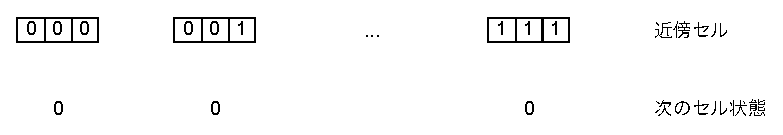
\includegraphics[width=8cm]{zu-ca.eps} \\
���륪���ȥޥȥ�(1����2��˵2����)���Ѳ���§�ΰ��\\
\end{tabular}
\caption{\label{zu-ca} [���륪���ȥޥȥ�]}
\end{center}
\end{figure}

セルオートマトンは、n次元のセル構造とセルの取り得る状態とセル状態の変化規則からなる。
例えば、「1次元3近傍2状態」とは、一次元に並ぶ有限または無限のセルと、変化規則が適応される3つの連続したセル(うち真ん中の一つは自分自身$=$状態変化の対象)のパターンからなる。
このとき、8通り($=2^3$)の状態からの遷移を規定しなければならず、すべての変化規則は256($=2^8$)通りとなる[Figure:\ref{zu-ca}]。
\begin{breakbox}$\Rightarrow$
2次元9近傍2状態の変化規則が何通りか考えよう。
\end{breakbox}

\subsection{プログラミングとは}
プログラミングとは、計算機に対しての処理命令をまとめたものであり、プログラミング言語はそれを行うための仕組みの一つである。
広義には、人間または計算機が、計算機に指示をするための様々なレベルの様々な仕組みであり、簡単なバッチ処理スクリプトや、たった一つの機械語命令もこれに含まれる。
しかし、より狭義には次のような特徴を持つプログラミング言語を用いて行うものが、プログラミングであると考えるのが妥当であろう。
\begin{itemize}
  \item 抽象化
  \item 繰り返しまたは再帰
  \item 条件分岐
\end{itemize}
抽象化とは、変数を利用可能であることである。ポインタの利用も抽象化の一種である。
繰り返しと再帰は、本質的に同等であり、相互に書き換えが可能であるとされる。
条件分岐は、最も直感的に必要であると考え得る機能のはずである。
\begin{breakbox}$\Rightarrow$
マークアップ言語(HTMLやYML)がプログラミング言語であり得るか、考えてみよう。
\end{breakbox}


